%%%%%%%%%%%%%%%%%%%%%%%%%%%%%%%%%%%%%%%%%%%%%%%%%%%%%%%%%%%%%%%%%%%%%
%
%  This is a sample LaTeX input file for your contribution to 
%  the MC2013 conference. Modified by R.C. Martineau at INL from A. 
%  Sood at LANL, from J. Wagner ORNL who obtained the original class 
%  file by Jim Warsa, LANL, 16 July 2002}
%
%  Please use it as a template for your full paper 
%    Accompanying/related file(s) include: 
%       1. Document class/format file: mc2013.cls
%       2. Sample Postscript Figure:   figure.eps
%       3. A PDF file showing the desired appearance: template.pdf 
%    Direct questions about these files to: richard.martinea@inl.gov
%
%    Notes: 
%      (1) You can use the "dvips" utility to convert .dvi 
%          files to PostScript.  Then, use either Acrobat 
%          Distiller or "ps2pdf" to convert to PDF format. 
%      (2) Different versions of LaTeX have been observed to 
%          shift the page down, causing improper margins.
%          If this occurs, adjust the "topmargin" value in the
%          mc2013.cls file to achieve the proper margins. 
%
%%%%%%%%%%%%%%%%%%%%%%%%%%%%%%%%%%%%%%%%%%%%%%%%%%%%%%%%%%%%%%%%%%%%%


%%%%%%%%%%%%%%%%%%%%%%%%%%%%%%%%%%%%%%%%%%%%%%%%%%%%%%%%%%%%%%%%%%%%%
\documentclass{mc2013}
%
%  various packages that you may wish to activate for usage 
\usepackage{graphicx}
\usepackage{tabls}
\usepackage{afterpage}
\usepackage{cites}
\usepackage{amssymb}
\usepackage{amsfonts}
\usepackage{amsmath}
\usepackage{amsthm}
\usepackage[mathcal]{euscript}

%\usepackage{epsf}
%
%
% Insert authors' names and short version of title in lines below
%
\newcommand{\authorHead}      % Author's names here
   {Slattery, Wilson, and Pawlowski}  
\newcommand{\shortTitle}      % Short title here
   {Data Transfer Kit}  
%%%%%%%%%%%%%%%%%%%%%%%%%%%%%%%%%%%%%%%%%%%%%%%%%%%%%%%%%%%%%%%%%%%%%
%
%   BEGIN DOCUMENT
%
%%%%%%%%%%%%%%%%%%%%%%%%%%%%%%%%%%%%%%%%%%%%%%%%%%%%%%%%%%%%%%%%%%%%%
\begin{document}

%
%      Headers and Footers
\afterpage{%
\fancyhf{}%
\fancyhead[CE]{              
{\scriptsize \authorHead}}                                                
\fancyhead[CO]{               
{\scriptsize \shortTitle}}                  
%\lfoot{\scriptsize{
%International Conference on Mathematics and Computational Methods
%Applied to Nuclear Science \& Engineering (M\&C 2013), 
%\\ Sun Valley, Idaho, USA, May 5-9, 2013.}}%
\rfoot{\thepage/\totalpages{}}%

\pagestyle{fancy}
%\setlength{\topmargin}{-20pt}
}
 
\normalsize

\setlength{\baselineskip}{16.8pt}
\vspace{-3pt}

% 
% TITLE
%

\begin{center}
\textbf{\large \\%
THE DATA TRANSFER KIT: A GEOMETRIC RENDEZVOUS-BASED TOOL FOR
MULTIPHYSICS DATA TRANSFER
}
% 
% FIRST AUTHORS 
%
\\
\setlength{\baselineskip}{14pt}
\textbf{S.R. Slattery and P.P.H. Wilson} \\
Department of Engineering Physics \\
University of Wisconsin - Madison \\
1500 Engineering Dr., Madison, WI 53706 \\
sslattery@wisc.edu; wilsonp@engr.wisc.edu \\

% 
% SECOND AUTHORS (if not needed delete from here) 
%
\vspace{12pt}
\textbf{R.P. Pawlowski}\\
Sandia National Laboratories \\
1515 Eubank SE, Albuquerque, NM 87123 \\
rppawlo@sandia.gov \\ 
%
% SECOND AUTHORS (to here)
%

\end{center}

%
% SET RAGGED RIGHT MARGIN
%
\raggedright


%%---------------------------------------------------------------------------%%
\section*{ABSTRACT} 
\begin{quote}
\begin{small}
The Data Transfer Kit (DTK) is a software component designed to
provide parallel services for data transfer for arbitrary physics
components based on the concept of geometric rendezvous. The
rendezvous algorithm provides a means to geometrically correlate two
geometric domains that may be arbitrarily decomposed in a parallel
simulation. By repartitioning both domains such that they have the
same geometric domain on each parallel process, efficient and load
balanced search operations and data transfer can be performed at a
desirable algorithmic time complexity with low communication overhead
relative to other types of mapping algorithms. With the increased
development efforts in multiphysics simulation and other multiple mesh
and geometry problems, generating parallel topology maps for
transferring fields and other data between geometric domains is a
common operation. This document describes the algorithms used to
generate parallel topology maps based on the concept of geometric
rendezvous as implemented in DTK with examples using a conjugate heat
transfer calculation and thermal coupling with a surrogate neutronics
code. In addition, we provide the results of initial scaling studies
performed on the Jaguar Cray XK6 system at Oak Ridge National
Laboratory for a worse-case-scenario problem in terms of algorithmic
complexity that shows good scaling on O(10,000) cores.


\emph{Key Words}: data transfer, multiphysics, rendezvous, parallel
computing
\end{small} 
\end{quote}

\setlength{\baselineskip}{14pt}
\normalsize

%%---------------------------------------------------------------------------%%
\Section{INTRODUCTION} 
\label{sec:intro}

In many physics applications, it is often desired to transfer fields
(i.e. degrees of freedom or other data) between geometric domains that
may or may not conform in physical space. In addition, for massively
parallel simulations, it is typical that geometric domains not only do
not conform spatially, but also that their parallel decompositions do
not correlate and are independent of one another due to physics-based
partitioning and discretization requirements. As an example, this
situation can occur in multiphysics simulations where physics fields
provide feedback between solution iterations or adaptive mesh
simulations where fields must be moved between meshes after refining
and coarsening. It is therefore desirable to have a set of tools to
relate two geometric domains of arbitrary parallel decomposition such
that fields and other data can be transferred between them.

Relating two non-conformal geometric domains will ultimately require
some type of function evaluation algorithm to apply the data from one
geometry to another. To drive these evaluation algorithms, the target
objects to which this data will be applied must be located within the
the source geometry. In a serial formulation, efficient search
structures that offer logarithmic asymptotic time complexity are
available to perform this operation. However, in a parallel
formulation, if these two geometries are arbitrarily decomposed,
geometric alignment is not likely and a certain degree of
communication will be required. A geometric rendezvous manipulates the
source and target geometries such that all geometric operations have a
local formulation.

The Data Transfer Kit (DTK) is a software component devloped as part
of the Consortium for Advanced Simulation of LWR's (CASL)
\cite{u.s._department_of_energy_casl_2011} designed to provide
parallel services for mesh and geometry searching and data transfer
based on the concept of geometric rendezvous as developed by Plimpton,
Hendrickson, and Stewart \cite{Plimpton_2004}. Their work has been
extended to move towards a component design for use with arbitrary
physics codes with general concepts of mesh, geometry, and fields are
employed to provide access to these services \cite{Chand_2008}. In
addition, their rendezvous algorithms have been expanded to be used
with both mesh and geometry representations of the geometric
domain. This document will briefly outline the rendezvous algorithms
as implemented in DTK. Examples of data transfer using a conjugate
heat transfer calculation and a CFD-neutronics type coupling are
provided. Parallel scaling results are also presented for the
point-to-point mapping algorithm for a worse-case-scenario problem
where communication costs are at a maximum.


%%---------------------------------------------------------------------------%%
\Section{RENDEZVOUS ALGORITHMS} 
\label{sec:rendezvous_algorithms}

A set of algorithms based on geometric rendezvous are implemented
within DTK. The purpose of these algorithms is to efficiently generate
a parallel topology map and the associated parallel communication plan
that can carry out the data transfer repeatedly with the minumum
required number of parallel messages and and data. A parallel topology
map is an operator, $M$, that defines the translation of a field,
$F(s)$, from a source spatial and parallel domain, $\Omega_S$, to a
field, $G(t)$, in the target spatial and parallel domain $\Omega_T$,
such that $M: \mathbb{R}^D \rightarrow \mathbb{R}^D, \forall r \in
[\Omega_S \cap \Omega_T]$, using both geometric and parallel
operations.

\Subsection{Point-to-Point Mapping}
\label{subsec:point_to_point}

Point-to-point mapping consists of interpolating data bound to a mesh
onto a point using the functions that represent the discretization of
the data over that mesh. For the mapping to access the required
physics data, fields will be required to be evaluated at points in
discrete domains. The actual discretization of the field is not
explicitly formulated. Rather, access to discretization of fields and
the associated data is generated through function evaluations at
points in physical space. Consider a $D$-dimensional function $F(r)$
of arbitrary discretization over the spatial domain $\Omega \in
\mathbb{R}^n$ where $r \in \mathbb{R}^n$ and $F : \mathbb{R}^n
\rightarrow \mathbb{R}^D$. Via polynomial interpolation, projection,
or any other means necessary to most appropriately reflect the
discretization of $F(r)$, it then follows that evaluation operations
of the following type can be performed:

\begin{equation}
  \hat{f} \leftarrow F(\hat{r}), \forall \hat{r} \in \Omega
  \label{eq:evaluation}
\end{equation}

where $\hat{r} \in \mathbb{R}^n$ is a single point and $\hat{f} \in
\mathbb{R}^D$ is representative of the function $F(r)$ evaluated at
$\hat{r}$. This operation is not valid for $\hat{r} \notin \Omega$. In
the context of $\Omega$ discretized by a geometric domains (such as
mesh elements or cylinders), these evaluations can instead be written
in terms of a single domain, $\omega \in \Omega$.

\begin{equation}
  \hat{f} \leftarrow F(\hat{r}), \forall \hat{r} \in \omega
  \label{eq:element_evaluation}
\end{equation}

This operation is then not valid for $\hat{r} \notin \omega$. If
$\hat{r} \notin \omega$ and $\hat{r} \notin \Omega$, then alternative
schemes may be chosen, such as extrapolation, in order to apply the
field to $\hat{r}$.


\Subsection{Volume-to-Volume Mapping}
\label{subsec:volume_to_volume}

\Subsection{Integral-to-Volume Mapping}
\label{subsec:integral_to_volume}


%%---------------------------------------------------------------------------%%
\Section{DATA TRANSFER EXAMPLES}
\label{sec:examples}

\Subsection{Conjugate Heat Transfer}
\label{subsec:cht}

\Subsection{CFD-Neutronics}
\label{subsec:cfd_neutronics}

%%---------------------------------------------------------------------------%%
\Section{SCALING STUDY}
\label{sec:scaling_study}

A typical use case of DTK is searching a mesh with a set of points and
applying field data to those points through function evaluations. For
this use case, a scaling study of the initial DTK implementation of
the rendezvous algorithm for data transfer was performed utilizing the
Jaguar Cray XK6 system at Oak Ridge National Laboratory. For each
study, a tri-linear hexahedron mesh was generated and decomposed
across the parallel domain. Figure~\ref{fig:mesh_partition} shows an
example of a mesh partition used in the scaling studies. Each
partition had one element in the z direction while the x and y
directions were varied to produce the desired number of elements in
the partition. All partitions in each scaling study are square. This
mesh is searched with random points generated by sampling the x and y
directions across the global mesh domain.  By striding the random
number seed used to generate the point coordinates, each process will
have a unique set of random points it is searching for. For each
scaling study, every process generated the same number of random
points as the number of elements on that process, ensuring that a
dense, all-to-all communication operation will be required for mapping
and data transfer. Once the points are mapped to the mesh, the data
transfer routine applies the process rank in which they were found and
transfers it back to the original owning process for the point. In
this way, because of the simple partitioning used for the scaling
studies, the results of the data transfer to the random points can be
independently verified by checking the applied data against the
expected mesh process rank.

\begin{figure}[htpb!]
  \centering 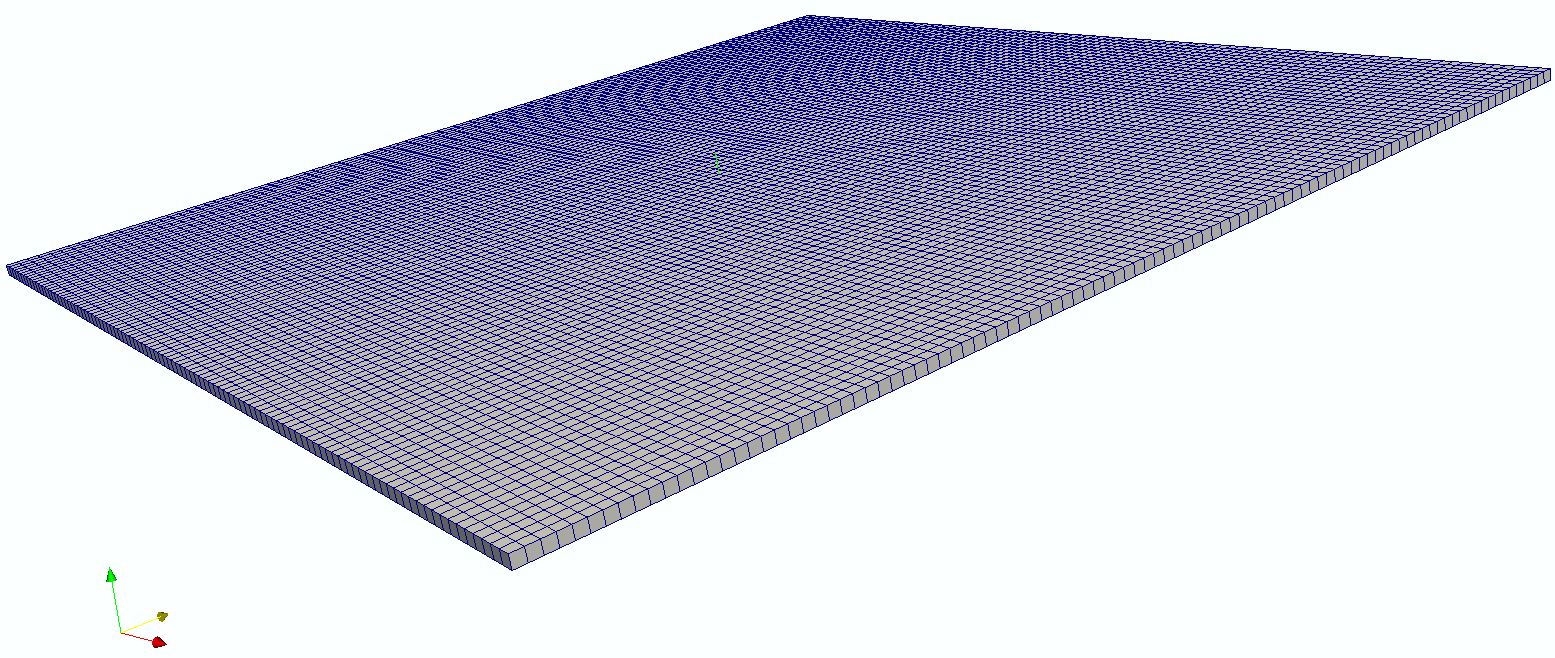
\includegraphics[width=4.5in]{mesh.png}
  \caption{\sl Local mesh partition for scaling studies. This
    particular mesh partition has 1.0E4 tri-linear hexahedrons.}
  \label{fig:mesh_partition}
\end{figure}

A weak scaling study was performed by fixing the problem size per core
and increasing the number of cores used while a strong scaling study
was performed by fixing the total problem size while increasing the
number of cores used.

\Subsection{Weak Scaling}
\label{subsec:weak_scaling}
For the weak scaling study, the number of hexahedrons per partition
was fixed to 1.0E4 and the number of random points generated per
partition also fixed to 1.0E4. The number of cores used varied from 16
to 65,536. Figure~\ref{fig:weak_scaling} gives the results of the weak
scaling study. It is clear from the weak scaling study that at high
numbers of processors communication latency begins to dominate for
this dense all-to-all problem as described above. However, it is worth
noting that once the mapping is complete, wall time for the actual
transfer of the data is several orders of magnitude less.

\begin{figure}[htpb!]
  \centering
  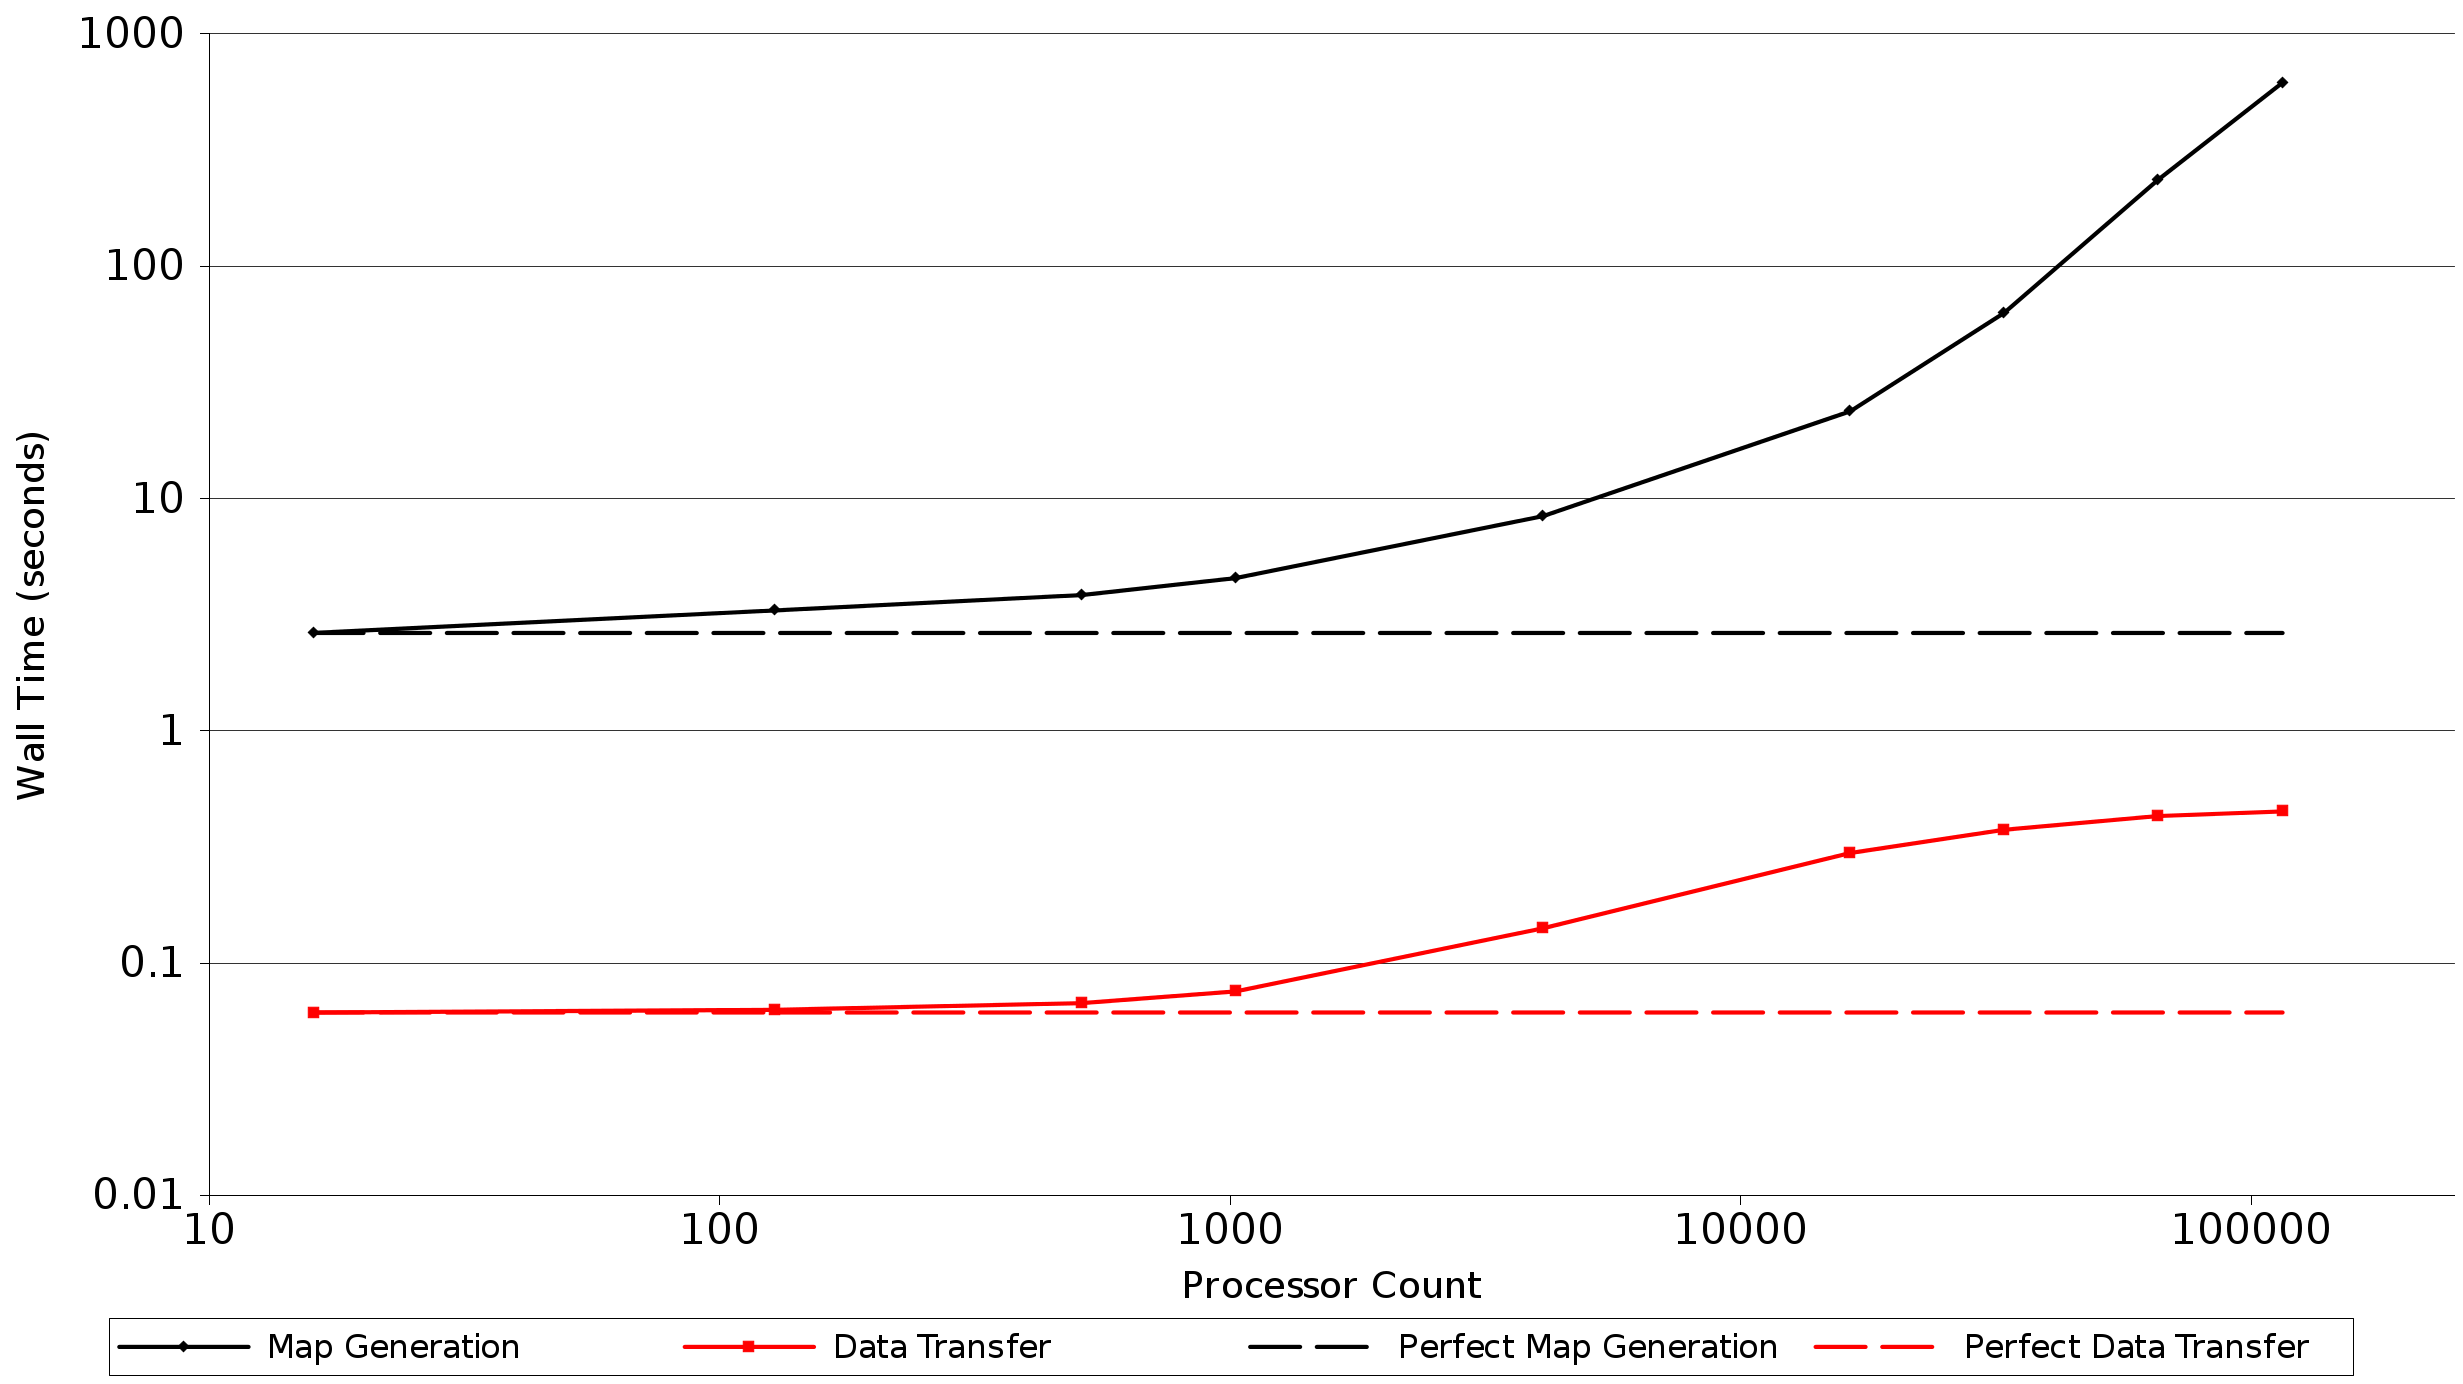
\includegraphics[width=5.5in]{WeakScaling.png}
  \caption{\sl Weak scaling study results. The blue curve reports the
    wall time to generate the mapping (setup) vs. number of processors
    while the red curve reports the wall time to transfer the data
    (apply) vs. number of processors. The dashed lines give perfect
    weak scaling. Note that both axes are on a logarithmic scale. }
  \label{fig:weak_scaling}
\end{figure}

Table~\ref{tab:weak_scaling}. Gives the raw data for the weak scaling
study. We note here that both the setup time (mapping) and the apply
time (data transfer) are relatively load balanced with average compute
times reported near the maximum compute time. In addition it should be
noted that for even the largest case at 65,536 cores the wall time is
not prohibitively large with the setup routine requiring approximately
13.6 minutes and the apply routine requiring less than half a second.

The efficiency values for the apply and setup routines are also
reported in table~\ref{tab:weak_efficiency} with the 16 core case used
as the reference computation. In correlation with the data presented
in table~\ref{tab:weak_scaling}, the efficiencies are observed to be
low above 1,000 cores for this dense all-to-all communication
problem. For more physical coupling problems where the communication
is expected to be much sparser, this gives and idea of just how sparse
that communication must be for this algorithm to scale well.

\begin{table}[htpb!]
  \begin{center}
    \begin{tabular}{llllllll}\hline\hline
      \multicolumn{1}{l}{} & 
      \multicolumn{1}{l}{Global} & 
      \multicolumn{1}{l}{Setup} & 
      \multicolumn{1}{l}{Setup} & 
      \multicolumn{1}{l}{Setup} & 
      \multicolumn{1}{l}{Apply} & 
      \multicolumn{1}{l}{Apply} & 
      \multicolumn{1}{l}{Apply}\\
      \multicolumn{1}{l}{Procs} & 
      \multicolumn{1}{l}{Elements} & 
      \multicolumn{1}{l}{Min (s)} & 
      \multicolumn{1}{l}{Max (s)} & 
      \multicolumn{1}{l}{Average (s)} & 
      \multicolumn{1}{l}{Min (s)} & 
      \multicolumn{1}{l}{Max (s)} & 
      \multicolumn{1}{l}{Average (s)}\\ \hline\hline
      %%
16 &	1.600E+05 & 2.79 &	2.82 &	  2.807 &	0.05 & 0.07 &	0.062 \\
128 &	1.280E+06 & 3.71 &	3.77 &	  3.758 &	0.06 &	0.07 &	0.063 \\
512 &	5.120E+06 & 5.81 &	6.12 &	  6.088 &	0.06 &	0.08 &	0.067 \\
1024 &	1.024E+07 & 8.46 &	9 &       8.962 &	0.07 &	0.09 &	0.077 \\
4096 &	4.096E+07 & 24.72 &	26.7 &	  26.561 &	0.15 &	0.19 &	0.168 \\
16384 &	1.638E+08 & 87.37 &	94.93 &	  93.915 &	0.28 &	0.32 &	0.296 \\
32768 &	3.277E+08 & 211.5 &	225.96 &  221.903 &	0.36 &	0.4 &	0.382 \\
65536 &	6.554E+08 & 792.85 & 816.85	& 811.704 &	0.42 &	0.46 &	0.436 \\
      \hline\hline
    \end{tabular}
  \end{center}
  \caption{\sl Weak scaling study data with the local problem size
    fixed to 1.0E4 elements/points. All times reported in
    seconds. Minimum, maximum, and average timing values are global
    and computed using the results from all processes.}
  \label{tab:weak_scaling}
\end{table}

\begin{table}[htpb!]
  \begin{center}
    \begin{tabular}{lll}\hline\hline
      \multicolumn{1}{c}{Procs}& 
      \multicolumn{1}{c}{Setup Efficiency} & 
      \multicolumn{1}{c}{Apply Efficiency}\\\hline\hline
      128 &	0.747 &	0.985 \\
      512 &	0.461 &	0.927 \\
      1024 &	0.313 &	0.807 \\
      4096 &	0.105 &	0.371 \\
      16384 &	0.029 &	0.210 \\
      32768 &	0.012 &	0.163 \\
      65536 &	0.003 &	0.143 \\
      %%
      \hline\hline
    \end{tabular}
  \end{center}
  \caption{\sl Weak scaling efficiencies. The 16 process case was used
    as the reference case.}
  \label{tab:weak_efficiency}
\end{table}

Compared to the weak scaling results observed by Plimpton et. al. for
a similar dense communication problem \cite{Plimpton_2004}, these
results show the same qualitative behavior (see figure 7 in the
reference). As the Jaguar system improves on all aspects of machine
performance over those used in the 2004 work, it is expected that
larger problems may be solved before the bandwidth limiting behavior
is observed.

\Subsection{Strong Scaling}
\label{subsec:strong_scaling}
For the strong scaling study, the global number of hexahedrons was
fixed to 1.0E8 and the global number of points fixed to 1.0E8 as
well with the number of cores varied from 256 to
16,384. Figure~\ref{fig:strong_scaling} gives the results of the
strong scaling study. Again, we note for the all-to-all communication
pattern required to map the random points that latency again begins to
dominate when a few thousand cores are used. The raw data for this
study is presented in table~\ref{tab:strong_scaling}. We see again
that the algorithm is relatively load balanced with average compute
times near the maximum reported compute times for the setup
operation. Table~\ref{tab:strong_efficiency} gives the efficiencies
computed for the strong scaling study with the 256 processor case used
as the reference.

\begin{figure}[htpb!]
  \centering
  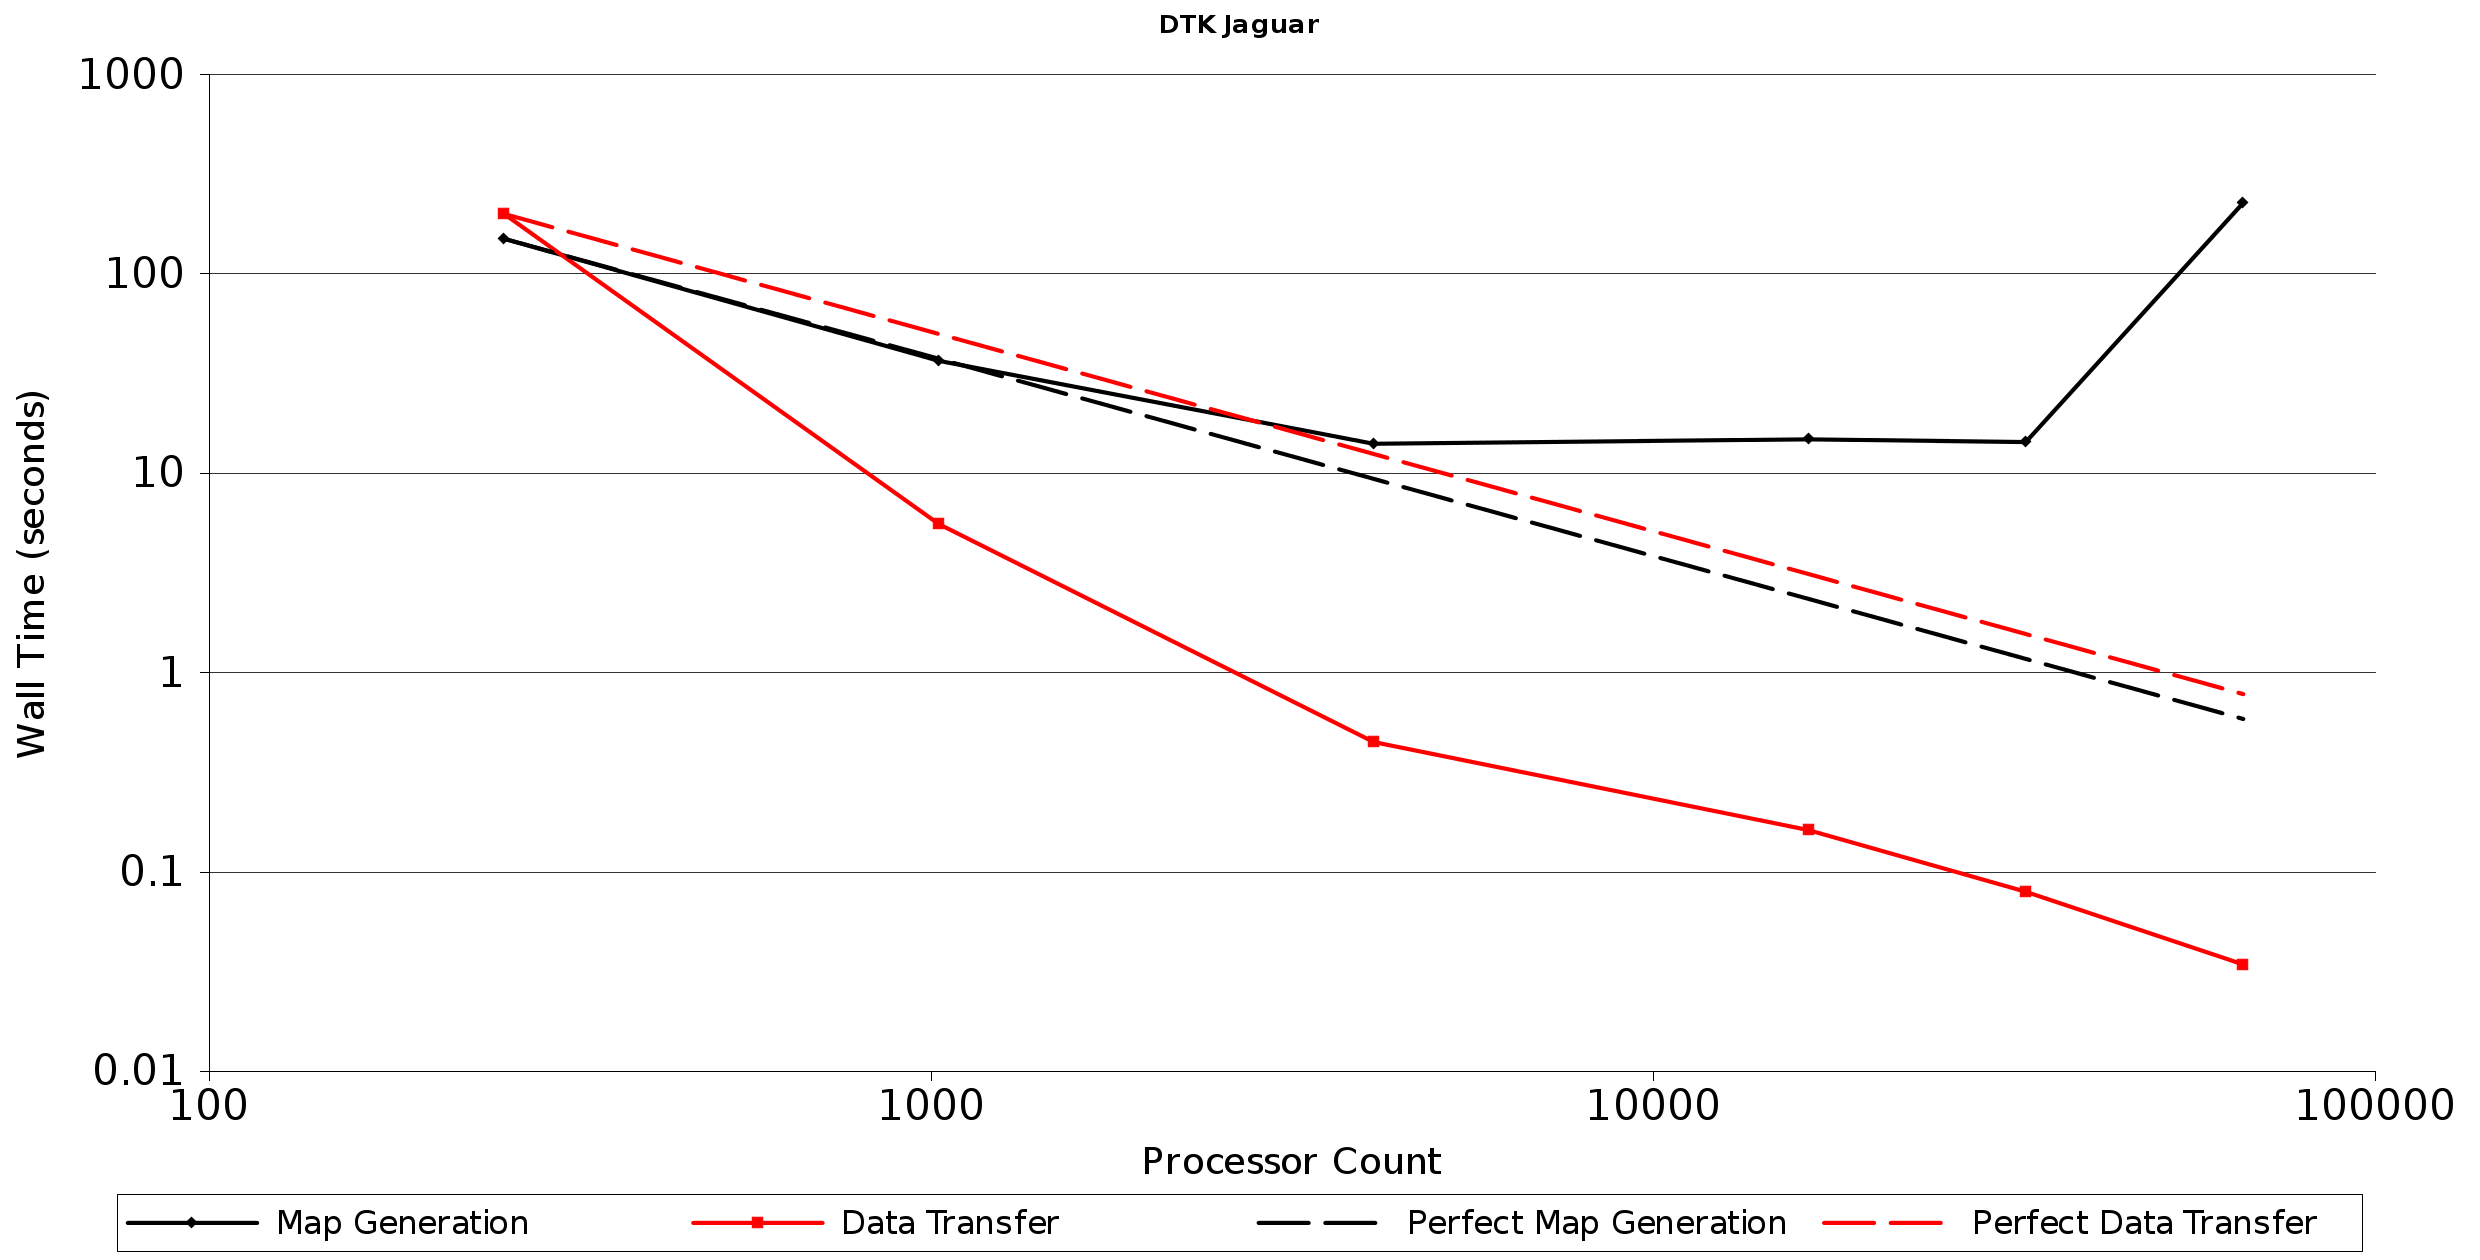
\includegraphics[width=5.5in]{StrongScaling.png}
  \caption{\sl Strong scaling study results with global problem size
    fixed to 1.024E7 elements/points. The blue curve reports the wall
    time to generate the mapping (setup) vs. number of processors
    while the red curve reports the wall time to transfer the data
    (apply) vs. number of processors. The dashed lines give perfect
    strong scaling. Note that the y-axis is a logarithmic scale. }
  \label{fig:strong_scaling}
\end{figure}

\begin{table}[htpb!]
  \begin{center}
    \begin{tabular}{llllllll}\hline\hline
      \multicolumn{1}{l}{}& 
      \multicolumn{1}{l}{Local} & 
      \multicolumn{1}{l}{Setup} & 
      \multicolumn{1}{l}{Setup} & 
      \multicolumn{1}{l}{Setup} & 
      \multicolumn{1}{l}{Apply} & 
      \multicolumn{1}{l}{Apply} & 
      \multicolumn{1}{l}{Apply}\\
      \multicolumn{1}{l}{Procs} & 
      \multicolumn{1}{l}{Elements} & 
      \multicolumn{1}{l}{Min (s)} & 
      \multicolumn{1}{l}{Max (s)} & 
      \multicolumn{1}{l}{Average (s)} & 
      \multicolumn{1}{l}{Min (s)} & 
      \multicolumn{1}{l}{Max (s)} & 
      \multicolumn{1}{l}{Average (s)}\\ \hline\hline
      %%
256 &	4.00E+04 & 17.66 &	17.77 &	17.748 & 0.93 &	0.96 &	0.944 \\
1024 &	1.00E+04 & 8.35 &	8.92 &	8.877 &	0.07 &	0.09 &	0.079 \\
4096 &	2.50E+03 & 7.02 &	8.14 &	8.067 &	0.03 &	0.05 &	0.038 \\
16384 &	6.25E+02 & 6.23 &	10.52 &	10.202 & 0 &	0.03 &	0.112 \\
      \hline\hline
    \end{tabular}
  \end{center}
  \caption{\sl Strong scaling study data. All times reported in
    seconds. Minimum, maximum, and average timing values are global
    and computed using the results from all processes.}
  \label{tab:strong_scaling}
\end{table}

\begin{table}[htpb!]
  \begin{center}
    \begin{tabular}{lll}\hline\hline
      \multicolumn{1}{c}{Procs}& 
      \multicolumn{1}{c}{Setup Efficiency} & 
      \multicolumn{1}{c}{Apply Efficiency}\\\hline\hline
      %%
      1024 &	0.498 &	2.984 \\
      4096 &	0.136 &	1.545 \\
      16384 &	0.026 &	0.131 \\
      \hline\hline
    \end{tabular}
  \end{center}
  \caption{\sl Strong scaling efficiencies. The 16 process case was used
    as the reference case.}
  \label{tab:strong_efficiency}
\end{table}

Again, compared to the work of Plimpton and his colleagues, this weak
scaling behavior for this type of problem is expected (see figure 6 in
the reference).  At a large enough number of processors, the bandwidth
limitations force the wall time to increase as the number of cores is
increased. As expected, this bandwidth limiting behavior is observed
at a larger problem size and number of cores than was observed in 2004
due to the improved computational resources available.

In addition to renewed weak and strong scaling studies, the largest
fixed processor run from the previous implementation was repeated at
16,384 cores with nearly 1.5 billion elements. Wall time for the setup
operation was reduced from 12.5 minutes to 1.26 minutes with apply
times approximately the same.


%%---------------------------------------------------------------------------%%
\Section{CONCLUSIONS}

We have presented the Data Transfer Kit, a new tool for massively
parallel data transfer for multiphysics applications. The concept of
geometric rendezvous is used to provide a collection of mesh and
geometry-based mappings for data transfer in shared domain problems.
Initial scaling studies have been completed for the Data Transfer Kit
on the Jaguar system. Their results show comparable qualitative
behavior to the literature results with improved performance due to
the more advanced computational resources available. However, for the
dense communication patterns required to complete the scaling study
problem, poor weak scaling results are still observed above O(10,000)
cores.

It is expected for more physical data transfer problems that the
communication pattern will be significantly sparser than the problem
presented here. Because of this, scaling is expected to improve for
more physical problems. Further scaling studies will be required to
test this hypothesis. In addition, the code has the potential to be
extended to provide surface-to-surface mappings for interface data
transfers.


%%---------------------------------------------------------------------------%%
\section*{ACKNOWLEDGEMENTS}

This work was performed under funding provided by the Consortium for
Advanced Simulation of Light Water Reactors (CASL). The authors would
like to the the CASL Virtual Reactor Integration (VRI) development
team for their assistance over the course of development of DTK and
the Oak Ridge Leaderership Computing Facility (OLCF) for providing
computational resources and support.

%%---------------------------------------------------------------------------%%
%\Section*{REFERENCES}
\setlength{\baselineskip}{12pt}
\bibliographystyle{ieeetr}
\bibliography{references}

\end{document}


